\section{线性回归}
\label{sec:regression-linear}

预测房价的一个起点，是给输入特征各配一个参数，用它们的加权和表示整体趋势。要由数据选出参数，先要规定什么误差值得减小，以及多大的参数变化可以接受。普通最小二乘用平方残差评价拟合；观测精度不同或误差相关时，加权与广义最小二乘调整残差的度量；特征彼此高度相关时，带惩罚项的目标收缩或选择参数，主成分回归与偏最小二乘则先改换回归方向；异常响应、非对称代价与容忍误差分别引出Huber回归、分位数回归与支持向量回归。原始特征的线性关系不足时，基函数回归、MARS与核岭回归改变输入表示；响应的取值范围与分布特征，则由广义线性模型与广义可加模型处理。

本节各模型都保留“对特征作全局线性加权”的骨架，只在三个环节上改变它：误差怎样计分、参数怎样受约束、特征或响应结构怎样表示。这些环节可以组合，下面按“先建立平方拟合，再依次改变误差度量、参数约束、回归方向、残差目标、特征表示与响应结构”的顺序展开，最后在第\ref{sec:regression-linear-relation}节把它们放在一起比较。

\subsection{普通最小二乘（OLS）}
\label{sec:regression-ols}

同一输入可能对应不同的观测响应，因而很难找到一条穿过所有样本的直线。先看一个教学例子：$x=0$处的响应为$2,4$，$x=1$处的响应为$4,6$。两处各有两个不同数值，精确插值已经不可能；若用平方残差计分，两个位置分别取均值$3,5$最合适，对应直线$f(x)=3+2x$。\term{普通最小二乘}（ordinary least squares, OLS）把这种选择推广为：在仿射函数族中寻找残差平方和最小的参数。平方损失让正、负误差受到相同惩罚，也让大误差付出更高代价。它可以作为无需指定响应分布的拟合准则；在独立、零均值且同方差的高斯误差下，又可解释为最大似然估计\scite{bishop2006}。

\subsubsection{模型结构}
\label{sec:regression-ols-structure}

设输入$\bm{x}\in\mathbb{R}^{d}$，数值响应$y\in\mathbb{R}$。预测取原始输入上的仿射函数
\begin{equation}
  f(\bm{x})=b+\bm{w}^{\top}\bm{x},
  \label{eq:regression-ols-model}
\end{equation}
其中$b$为截距，$\bm{w}\in\mathbb{R}^{d}$为斜率参数。OLS采用平均半平方目标
\begin{equation}
  (\widehat{\bm{w}},\widehat b)
  \in\argmin_{\bm{w},b}\ J(\bm{w},b),
  \qquad
  J(\bm{w},b)=\frac{1}{2n}\sum_{i=1}^{n}
    \bigl(y_i-b-\bm{w}^{\top}\bm{x}_i\bigr)^2,
  \label{eq:regression-ols-objective}
\end{equation}
因子$1/(2n)$不改变最优解，只是把梯度写成单记录误差的平均，后续梯度与更新都沿用这一约定。

图\ref{fig:regression-ols-residuals}把这个目标放回输入与响应平面：每条虚线都是固定$x_i$之后，观测$y_i$与直线预测之间的纵向差。OLS选择让这些响应方向上的差的平方和最小的直线，因此拟合线通常不穿过每个样本；图中的距离沿响应轴测量，区别于点到直线的垂直几何距离。

\begin{figure}[htbp]
  \centering
  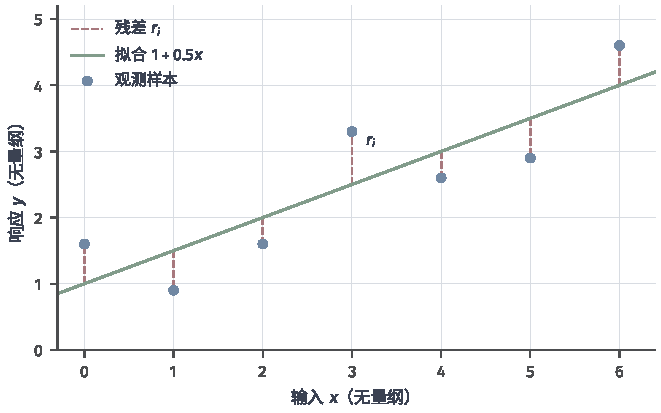
\includegraphics[width=105.412mm]{figures/04-classic-models/00-shared/matplotlib/regression-ols-residuals/figure.pdf}
  \caption{一维OLS与响应残差。七个构造样本的最小二乘直线为$\widehat f(x)=1+0.5x$；蓝色实心点表示观测，绿色实线表示预测，红色竖虚线表示$r_i=y_i-\widehat f(x_i)$。横、纵轴均为无量纲教学变量。}
  \label{fig:regression-ols-residuals}
\end{figure}

\subsubsection{参数学习}
\label{sec:regression-ols-learning}

\paragraph{显式梯度与参数更新}

对式\eqref{eq:regression-ols-objective}求导：每条记录$(y_i-b-\bm{w}^{\top}\bm{x}_i)^2$对$\bm{w}$的导数为$-2(y_i-b-\bm{w}^{\top}\bm{x}_i)\bm{x}_i$、对$b$的导数为$-2(y_i-b-\bm{w}^{\top}\bm{x}_i)$，除以$2n$后
\[
  \nabla_{\bm w}J
  =\frac1n\sum_{i=1}^{n}\bigl(b+\bm{w}^{\top}\bm{x}_i-y_i\bigr)\bm{x}_i,
  \qquad
  \frac{\partial J}{\partial b}
  =\frac1n\sum_{i=1}^{n}\bigl(b+\bm{w}^{\top}\bm{x}_i-y_i\bigr).
\]
两个梯度用同一轮参数计算。沿负方向按步长$\eta$迭代：
\begin{align}
  \bm{w}^{(t+1)}
  &=\bm{w}^{(t)}-\frac{\eta}{n}\sum_{i=1}^{n}\bigl(b^{(t)}+\bm{w}^{(t)\top}\bm{x}_i-y_i\bigr)\bm{x}_i,\\
  b^{(t+1)}
  &=b^{(t)}-\frac{\eta}{n}\sum_{i=1}^{n}\bigl(b^{(t)}+\bm{w}^{(t)\top}\bm{x}_i-y_i\bigr).
  \label{eq:regression-ols-gradient}
\end{align}
以教学例验证：$\widehat b=3$、$\widehat w=2$时，四项$b+wx_i-y_i$分别为$3+0-2=1$、$3+0-4=-1$、$3+2-4=1$、$3+2-6=-1$；$\partial J/\partial b=(1-1+1-1)/4=0$，$\nabla_{\bm w}J$中各项乘$x_i$后为$0,0,1,-1$，和为零，偏导数确实在该处为零。梯度置零给出的线性方程组可一次解出闭式参数。

\subsubsection{理论分析}
\label{sec:regression-ols-theory}

\paragraph{平方损失与条件均值}

到现在为止，平方残差只评价已经观测到的记录。真正要预测的是下一条记录：把未来输入与其响应看作同一总体中的随机变量$(\bm X,Y)$。设$\mathbb{E}[Y^2]<\infty$，并考察平方可积的预测函数$f$。固定一个未来输入$\bm X=\bm x$（$\bm x$是一组具体的房屋属性，不必是训练集中出现过的记录），响应$Y$仍会围绕某一平均水平波动，记条件均值$m(\bm x)=\mathbb{E}[Y\mid\bm X=\bm x]$为该属性组合下的平均响应。拟合直线的目的，就是让$f(\bm x)$尽量靠近这条$m(\bm x)$。

在$\bm X=\bm x$处，把任意预测$a$与条件均值的偏差拆成两段：
\[
  Y-a=(Y-m(\bm x))+(m(\bm x)-a).
\]
第一段是响应绕自身均值的波动，第二段是预测瞄得准不准。平方后交叉项$\mathbb{E}[(Y-m(\bm x))(m(\bm x)-a)\mid\bm X=\bm x]=(m(\bm x)-a)\mathbb{E}[Y-m(\bm x)\mid\bm X=\bm x]=0$——条件均值处的波动平均为零，两段不再纠缠，于是
\[
  \mathbb{E}[(Y-a)^2\mid\bm X=\bm x]
  =\operatorname{Var}(Y\mid\bm X=\bm x)+[m(\bm x)-a]^2.
\]
第一项是固定输入后响应自身的波动，任何预测函数都消不掉，即不可约噪声；第二项在$a=m(\bm x)$时取零。按未来输入的分布平均后，最小化期望平方损失的预测函数就是条件均值$m(\bm x)$；这个结论不要求高斯性或同方差性，可参考\BookChapterRef{chap:random-variables}{卷2《数学准备：概率、因果与决策》的“随机变量与概率基础”章}。

定义预测$f$的平方风险为$R(f)=\frac12\mathbb{E}[(Y-f(\bm X))^2]$。由上面的分解，
\[
  R(f)-R(m)=\tfrac12\mathbb{E}\bigl[(f(\bm X)-m(\bm X))^2\bigr].
\]
OLS在所有仿射函数中最小化训练记录上的平均平方损失；若它学到的$f$接近$m$，这一超额风险就小。接近程度由两件事决定：真实$m$是否落在仿射类的表示范围内（表示能力），以及有限样本估出的参数围绕总体最佳仿射函数的抽样波动。训练平均损失与期望风险之间的一般关系，包括样本量与模型容量如何影响这一距离，由卷三的泛化理论系统处理，可参考\BookChapterRef{chap:statistical-learning-framework}{卷三《基础、理论与可信性》的“统计学习框架”章}。
